 %!TEX root = coexistence_paper.tex



\section{Handling Coexistence}\label{sec:coexistence}
  


 

In massive crowds of coexisting networks, the interference pattern can be hard to detect for an LPWAN device like LoRa .  Hence, a TDMA (time division multiple access) or traditional CSMA/CA based approach will simply fail. As the wireless environment is largely unknown due to the coexistence of a massive number of unknown devices/networks,  a {\slshape learning} based approach becomes more effective to make actions (e.g, transmit, sleep, backoff) according to the environmental conditions. However, a learning process usually can be time and computation extensive while the nodes are power-constrained and battery-operated. Hence, we propose to adopt a lightweight machine learning approach. Specifically, as the SNOW nodes may have no knowledge of the coexisting networks, we will adopt  {\bf\slshape Reinforcement Learning (RL)} that enables an {\slshape agent} (e.g., a node) to learn by interacting with its environment~\cite{RLBook}. As shown in Fig.~\ref{fig:reinforcement}, an agent regularly updates its achieved {\slshape rewards} based on the taken action at a given {\slshape state}.  It will learn to take the best actions that maximize its long-term rewards by using its own experience. This would be the {\bf first RL approach} for LPWAN and for handling coexistence for any low-power network. 



 
    \begin{figure}%{r}{4.2cm}
    \centering%\vspace{-0.6in}
    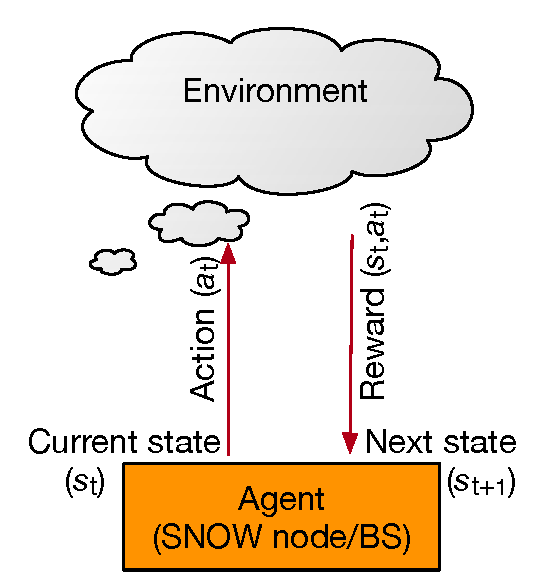
\includegraphics[width=0.22\textwidth]{figs/reinforcement.eps}      
    \vspace{-0.05in}
    \caption{\scriptsize RL visualization}\vspace{-0.1in}
    \label{fig:reinforcement}
 \end{figure}
 
 
\subsection{Rationale for Reinforcement Learning} 
 We adopt {\slshape Q-learning},  a widely-adopted RL technique, which is well-suited for coexistence handling because it is useful in decision making under unknown network conditions. It has {\slshape low memory requirements} and {\slshape low computation}, and learns  near-optimal or even {\slshape optimal} solution under certain conditions. Q-learning can be {\slshape efficiently} implemented in a distributed platform like WSN, where each node chooses actions to maximize rewards. It has been efficiently used in cognitive radios~\cite{cognitive1}, and in WSN for routing~\cite{RLRouting1, RLRouting2, RLRouting3, RLRouting4},  QoS provisioning~\cite{QoS1, QoS2}, and resource management \cite{RLSurvey}. It was also used with  RTS/CTS  to learn contention and collision with the nodes in the {\bf same} network  using a {\bf single channel}~\cite{RLMAC}.  SNOW exploits many subcarriers concurrently and does not rely on energy-consuming RTS/CTS frames. We aim to adopt RL to handle its coexistence with numerous  unknown and uncoordinated networks. RL has not yet been adopted to handle such coexistence. LPWAN technologies like LoRa or SNOW have unique features which require a new Q-learning framework. For example, LoRa networks enable multiple concurrent transmissions by dynamically adjusting multiple transmission parameters, whereas SNOW features massive concurrent communications on numerous narrowband subcarriers, white space dynamics, and PAPR constraints. Our Q-learning framework is able to dynamically leverage each of these unique characteristics to effectively handle co-existance. 
 
 
 %Adopting it for SNOW that features massive concurrent communications on numerous narrowband subcarriers, white space dynamics, PAPR constraints, and very low-power requires a new  Q-learning framework. 
   
%\subsection{Proposed Q-Learning Framework for SNOW}

%SNOW nodes will adopt Q-learning. The purpose of learning in nodes is to learn about the communication pattern of the coexisting networks. 
%On the BS side, this can help determine usable subcarriers and their use pattern.  The actions of a BS can also include load balancing among the subcarriers considering its outside utilization (in coexisting users). 
%To each node, we assign  prioritized access to multiple subcarriers. The intuition is that if one subcarrier is busy or noisy, another may remain free.
%A node will  start with its first priority subcarrier. If a subcarrier is busy,  it will either back-off or hop to its next subcarrier. If Tx fails on one subcarrier, a node can choose to retransmit on the same or the next prioritized subcarrier on a higher Tx power.  When a node has chosen a subcarrier it can either transmit on it, or backoff, or hop to the next priority subcarrier, or sleep. If some subcarriers become unavailable due to primary users, the nodes are informed using some backup subcarriers which is a common technique  in cognitive radios~\cite{ws_sigcomm09}. \revise{Nodes switch to backup subcarriers if no communication happens on their subcarriers for a certain time length.}  Since the BS can use fragmented spectrum, it can turn on and off some subcarriers based on their noise level. The Q-learning framework on the BS side will take into account the cost associated with PAPR in downlink communication. To reduce PAPR, it uses a subset of the Rx subcarriers on the Tx radio for sending ACKs. A node may need to transmit on one subcarrier and listen for ACK on another. The BS may put multiple ACKs on a subcarrier along with any subcarrier reassignment information. 


%    \begin{figure}%{r}{4.2cm}
  %  \centering%\vspace{-0.6in}
 %   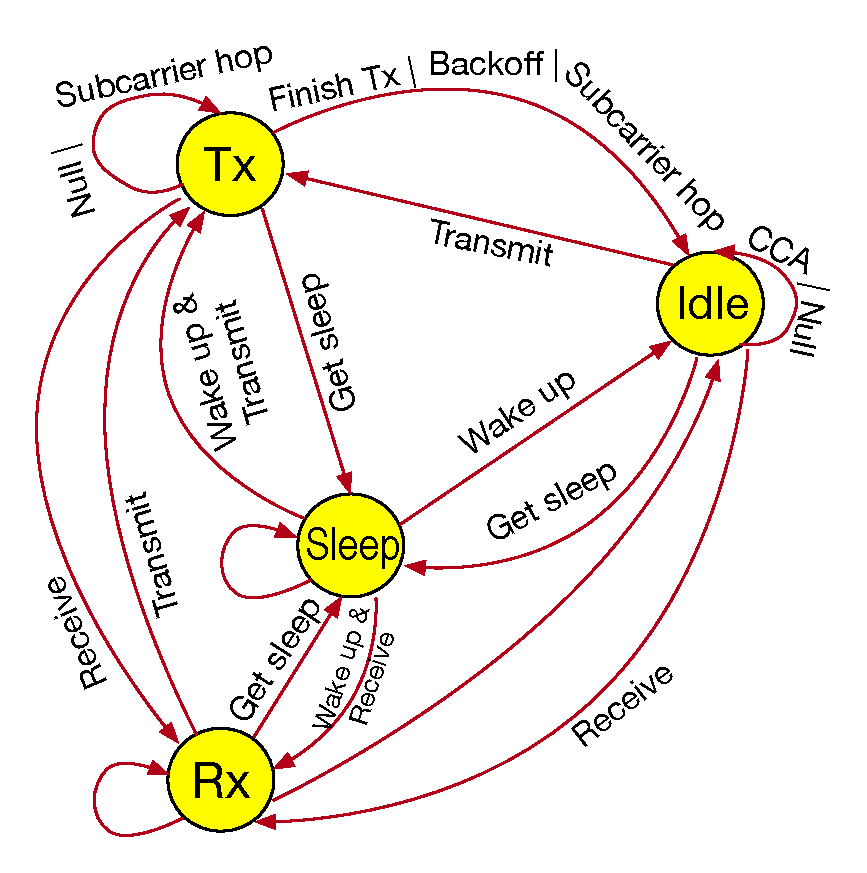
\includegraphics[width=0.33\textwidth]{figs/statediagram.eps}      
 %   \vspace{-0.05in}
 %   \caption{\scriptsize Agent state diagram}\vspace{-0.1in}
 %   \label{fig:statediagram}
%\end{figure}


%\noindent{\bf Reward Function Formulation for Node.}  Every SNOW node individually adopts Q-learning to make its decision. It adopts 
%{\slshape CCA (clear channel assessment)} for carrier sensing. Its set of actions is $\Lambda= \{ \text{\slshape \small Transmit, Receive, Backoff, Wake up, Subcarrier hop, CCA, Get sleep, null} \}$. We  consider agent (node) states $\Omega=\{\text{\slshape \small Tx, Rx, Idle, sleep}  \}$, to indicate its state of transmitting, receiving, idle,  sleeping.   Fig.~\ref{fig:statediagram} shows state transitions. Let $s_t\in \Omega$  be the agent state at time $t$. Its total reward is given by 
 % \vspace{-2mm}
 %$$
% \vspace{-2mm}
% R(s_t, a_t) = r(s_t, a_t) + c(s_t, a_t),$$
% where $r(s_t, a_t)$ is the {\slshape immediate reward}  and $c(s_t, a_t)$ is the {\slshape cost} of taking action $a_t\in \Lambda$  at state $s_t$. Considering both energy consumption and throughput, we can assign some numerical values indicating rewards and costs. As an example, we can consider total reward for a successful packet {\slshape transmission} or {\slshape reception} by considering 2 units of immediate reward  and 1 unit of cost. Thus, a failed transmission will incur only a cost of 1 unit. We can also consider 1 unit of cost in {\slshape idle} state (as the radio consumes energy almost similar to Tx/Rx). From $s_t=${\slshape Idle}, important reward functions can be given as follows. 
%\begin{footnotesize}

%$$%\vspace{-1mm}
%R(s_t, a_t) =
%\begin{cases}
%2 - 1 = 1   & \text{if }  s_t= \text{\slshape Idle},     ~a_t= \text{{\slshape Transmit} and ACK received}\\
%0 - 1 = -1   & \text{if } s_t= \text{\slshape Idle},     ~a_t= \text{{\slshape Transmit} and ACK not received}\\
%2 - 1 = 1   & \text{if } s_t= \text{\slshape Idle},     ~a_t= \text{\slshape Receive}\\
%- 1   & \text{if } s_t= \text{\slshape Idle},     ~a_t= \text{\slshape Null}\\
%- 1   & \text{if } s_t= \text{\slshape Idle},     ~a_t= \text{\slshape CCA}\\
%0   & \text{if } s_t= \text{\slshape Idle},     ~a_t= \text{\slshape Get sleep}
%\end{cases}
%$$\end{footnotesize}
%\revise{
%\begin{footnotesize}
%$$%\vspace{-1mm}
%R(s_t, a_t) =
%\begin{cases}
%2 - 1 = 1   & \text{if }  s_t= \text{\slshape Sleep},     ~a_t= \text{{\slshape Transmit} and ACK received}\\
%0 - 1 = -1   & \text{if } s_t= \text{\slshape Sleep},     ~a_t= \text{{\slshape Transmit} and ACK not received}\\
%2 - 1 = 1   & \text{if } s_t= \text{\slshape Sleep},     ~a_t= \text{\slshape Receive}\\
% 0   & \text{if } s_t= \text{\slshape Sleep},     ~a_t= \text{\slshape Null}\\
%-1   & \text{if } s_t= \text{\slshape Sleep},     ~a_t= \text{\slshape Wake up}
%\end{cases}
%$$\end{footnotesize}
%}

%\revise{
%\begin{footnotesize}
%$$%\vspace{-1mm}
%R(s_t, a_t) =
%\begin{cases}
%2 - 1 = 1   & \text{if }  s_t= \text{\slshape Tx},     ~a_t= \text{{\slshape Finish Tx} and ACK received}\\
%0 - 1 = -1   & \text{if } s_t= \text{\slshape Tx},     ~a_t= \text{{\slshape Finish Tx} and ACK not received}\\
%- 1   & \text{if } s_t= \text{\slshape Tx},     ~a_t= \text{{\slshape Backoff}}\\
%- 1   & \text{if } s_t= \text{\slshape Tx},     ~a_t= \text{{\slshape Subcarrier hop and remain Idle}}\\
%2 - 1 = 1   & \text{if } s_t= \text{\slshape Tx},     ~a_t= \text{{\slshape Subcarrier hop, transmit and ACK received}}\\
%- 1 = 1   & \text{if } s_t= \text{\slshape Tx},     ~a_t= \text{{\slshape Subcarrier hop, transmit and ACK not received}}\\
%2 - 1 = 1   & \text{if } s_t= \text{\slshape Tx},     ~a_t= \text{\slshape Receive}\\
%-1   & \text{if } s_t= \text{\slshape Tx},     ~a_t= \text{\slshape Null}\\
%0   & \text{if } s_t= \text{\slshape Tx},     ~a_t= \text{\slshape Get %Sleep}
%\end{cases}
%$$\end{footnotesize}
%}
%\revise{
%\begin{footnotesize}
%$$%\vspace{-1mm}
%R(s_t, a_t) =
%\begin{cases}
%2 - 1 = 1   & \text{if }  s_t= \text{\slshape Rx},     ~a_t= \text{{\slshape Finish Rx}}\\
%2 - 1 = 1   & \text{if } s_t= \text{\slshape Rx},     ~a_t= \text{{\slshape Transmit} and ACK received}\\
%0 - 1 = - 1   & \text{if } s_t= \text{\slshape Rx},     ~a_t= \text{{\slshape Transmit} and ACK not received}\\
%- 1   & \text{if } s_t= \text{\slshape Rx},     ~a_t= \text{{\slshape go to idle}}\\
%-1   & \text{if } s_t= \text{\slshape Rx},     ~a_t= \text{\slshape Null}\\
%0   & \text{if } s_t= \text{\slshape Rx},     ~a_t= \text{\slshape Get Sleep}
%\end{cases}
%$$\end{footnotesize}}
%\noindent \revise{Based on this idea, we need to formulate  all reward functions for a node agent...... }



%\noindent{\bf Reward Function Formulation for BS.} Here we provide an outline to formulate reward functions for the BS. 
%The BS will maintain states and actions for each subcarrier on both Rx radio and the Tx radio. For our preliminary formulation, we consider two states, Rx\_OFF and Rx\_ON, for each subcarrier on the Rx radio to indicate if it is ON or OFF. The actions are: {\slshape Turn Rx ON}, {\slshape Turn Rx OFF}, and {\slshape null}. We consider similar states and actions for each subcarrier on the Tx radio. A state diagram showing these states and actions is shown in Fig.~\ref{fig:sc_statediagram} for a subcarrier at the BS. For a subcarrier $f_i$ used in the Rx radio for receiving from the nodes, let {\bf rps}$(t,i)$ be packet rate (number of packets received per unit time) per subcarrier at time $t$ if we add subcarrier $f_i$ to the Rx radio.  Let {\bf lps}$(t,i)$ be loss rate (number of times the BS recognizes high signal strength on a subcarrier but cannot decode packet per unit time) per subcarrier at time $t$ if we add subcarrier $f_i$ to the Rx radio. Thus, rps$(t,i)$ and lps$(t,i)$ can be considered {\slshape reward} and {\slshape cost}, respectively, for turning $f_i$ on at the Rx radio. Let {\bf aps}$(t,i)$ be ACK rate (number of ACKs sent per unit time) per subcarrier at time $t$ if we add subcarrier $f_i$ to the Tx radio. Let $m_{\text{tx}} (t)$ be the total number of subcarriers used by the Tx radio for ACK at time $t$. If the BS's maximum tolerable PAPR is $\beta$, then if adding a subcarrier  exceeds this value, i.e.  if $m_{\text{tx}} (t)+1 > \beta$, we  consider a penalty (cost) as the BS has to dissipate more energy. Considering $\nu$ as some normalized cost per subcarrier,   R-values for subcarrier $f_i$ can be formulated as follows.





%\begin{small}
$$
%R(s^i_t, a^i_t) =
%\begin{cases}
%\text{rps} (t, i) - \text{lps} (t, i)  & \text{if }  s^i_t= \text{\slshape Rx\_OFF},     ~a^i_t= \text{{\slshape Turn Rx ON}}\\
%\text{aps} (t, i)   -     \frac{\max \big (0,   m_{\text{tx}} (t) +1  - \beta \big )}{\beta}   & \text{if }  s^i_t= \text{\slshape Tx\_OFF},     ~a^i_t= \text{{\slshape Turn Tx ON}}
%\text{aps} (t, i)   -   \nu . \max \big (0,   m_{\text{tx}} (t) +1  - \beta \big )  & \text{if }  s^i_t= \text{\slshape Tx\_OFF},     ~a^i_t= \text{{\slshape Turn Tx ON}}
%\end{cases}
$$
%\end{small}

%\noindent{\bf Reward Function Formulation for LoRa node.}
%to do..(may remain the same with snow node)

%\noindent{\bf Reward Function Formulation for LoRa BS.}
%LoRa gateways are half-duplex. Thus they can not receive and transmit at the same time. Moreover, a LoRa gateway can only transmit to an end device if it has received a transmission from it. If a LoRa gateway turns its transmission 
%\begin{small}
%$$
%R(s^i_t, a^i_t) =
%\begin{cases}
%\text{rps} (t, i) - \text{lps} (t, i)  & \text{if }  s^i_t= \text{\slshape TX\_ON},     ~a^i_t= \text{{\slshape Turn Rx ON}}\\
%\text{aps} (t, i)   -     \frac{\max \big (0,   m_{\text{tx}} (t) +1  - \beta \big )}{\beta}   & \text{if }  s^i_t= \text{\slshape Tx\_OFF},     ~a^i_t= \text{{\slshape Turn Tx ON}}
%\text{aps} (t, i)   -   \text{mps}(t,i)  & \text{if }  s^i_t= \text{\slshape Rx\_ON},     ~a^i_t= \text{{\slshape Turn Tx ON}}
%\end{cases}
%$$
%\end{small}


 
\subsection{Proposed Q-learning \edit{Frame work} for LoRa}
LoRa nodes will use Q-learning MAC for uplink communication. The Q-learning MAC aims to learn the communication pattern of other co-existing networks and take intelligent decisions to increase the network performance. Each node will start transmitting on a randomly selected channel from the set of enabled channels in the operating band. The network manager initially assigns spreading factors to nodes. Nodes start transmitting using the allocated spreading factors. However, nodes can change their channel and spreading factor after each transmission based on the Q-learning MAC. After each failed transmission,the nodes can choose to transmit in another channel, or transmit using another spreading factor or they can choose to not re-transmit immediately and back-off. 

 \begin{figure*}%[!htpb]%{r}{4.1cm}
    \centering%\hfill
    \subfigure[\footnotesize SNOW Node states\label{fig:statediagram}]{
     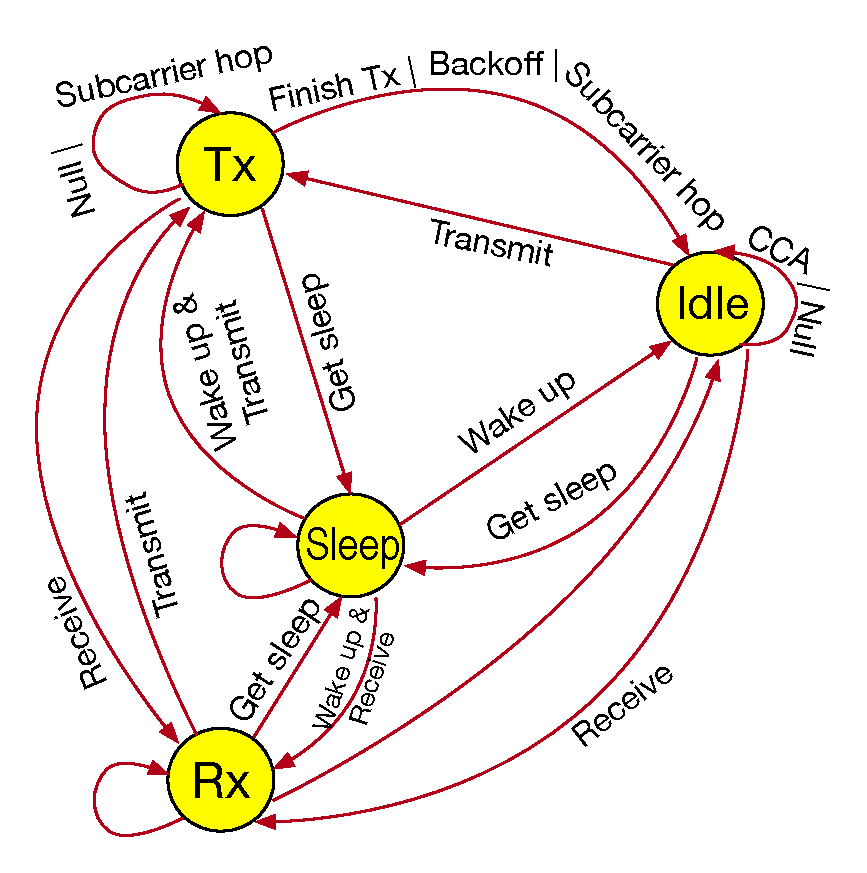
\includegraphics[width=.33\textwidth]{figs/statediagram.eps}
    } \hfill
    \subfigure[\footnotesize LoRa Node States states.\label{fig:statediagram_lora}]{
    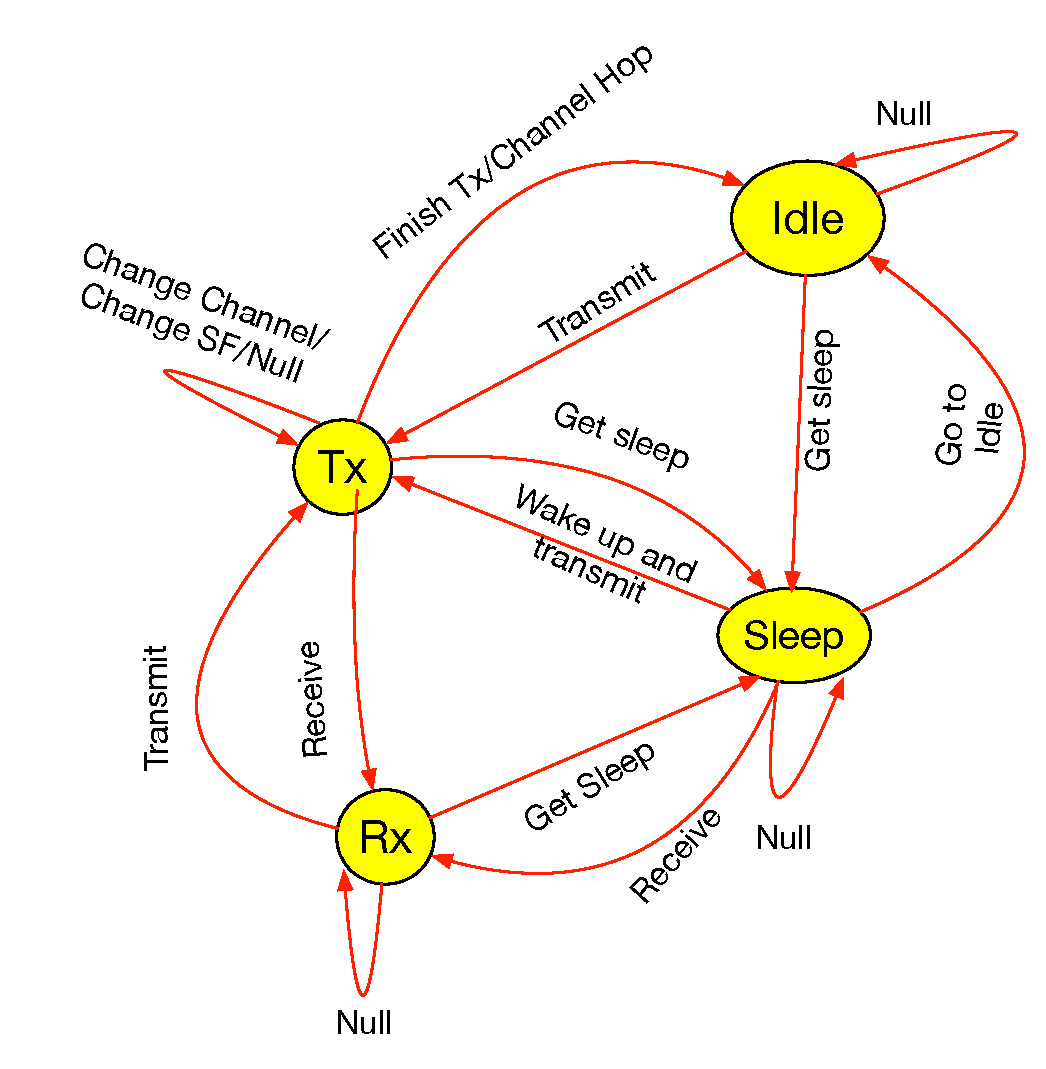
\includegraphics[width=0.4\textwidth]{figs/State_diagram_lora.eps}
      }
      \vspace{-0.15in}
    \caption{\footnotesize Agent state diagram.}%\vspace{-.15in}
   \label{fig:rl}
 \end{figure*}
 
 
Thus, the set of actions is
\vspace{-2mm}
 $$
  \vspace{-2mm}
  \Lambda=\{\text{\slshape \small Transmit, Receive, Backoff, Wake up, Channel hop, Change SF, Get sleep, null}\}$$
 We  consider agent (node) states $\Omega=\{\text{\slshape \small Tx, Rx, Idle, sleep}  \}$, to indicate its state of transmitting, receiving, idle,  sleeping. Based on this action set, the reward functions for LoRa nodes can be constructed as follows: 


\revise{
\begin{footnotesize}
$$%\vspace{-1mm}
R(s_t, a_t) =
\begin{cases}
2 - 1 = 1   & \text{if }  s_t= \text{\slshape Idle},     ~a_t= \text{{\slshape Transmit} and ACK received}\\
0 - 1 = -1   & \text{if } s_t= \text{\slshape Idle},     ~a_t= \text{{\slshape Transmit} and ACK not received}\\
2 - 1 = 1   & \text{if } s_t= \text{\slshape Idle},     ~a_t= \text{\slshape Receive}\\
- 1   & \text{if } s_t= \text{\slshape Idle},     ~a_t= \text{\slshape Null}\\
0   & \text{if } s_t= \text{\slshape Idle},     ~a_t= \text{\slshape Get sleep}
\end{cases}
$$\end{footnotesize}
}

\revise{
\begin{footnotesize}
$$%\vspace{-1mm}
R(s_t, a_t) =
\begin{cases}
2 - 1 = 1   & \text{if }  s_t= \text{\slshape Sleep},     ~a_t= \text{{\slshape Transmit} and ACK received}\\
0 - 1 = -1   & \text{if } s_t= \text{\slshape Sleep},     ~a_t= \text{{\slshape Transmit} and ACK not received}\\
2 - 1 = 1   & \text{if } s_t= \text{\slshape Sleep},     ~a_t= \text{\slshape Receive}\\
 0   & \text{if } s_t= \text{\slshape Sleep},     ~a_t= \text{\slshape Null}\\
-1   & \text{if } s_t= \text{\slshape Sleep},     ~a_t= \text{\slshape Wake up}
\end{cases}
$$\end{footnotesize}
}

\revise{
\begin{footnotesize}
$$%\vspace{-1mm}
R(s_t, a_t) =
\begin{cases}
2 - 1 = 1   & \text{if }  s_t= \text{\slshape Tx},     ~a_t= \text{{\slshape Finish Tx} and ACK received}\\
0 - 1 = -1   & \text{if } s_t= \text{\slshape Tx},     ~a_t= \text{{\slshape Finish Tx} and ACK not received}\\
- 1   & \text{if } s_t= \text{\slshape Tx},     ~a_t= \text{{\slshape Backoff}}\\
- 1   & \text{if } s_t= \text{\slshape Tx},     ~a_t= \text{{\slshape Channel hop and remain Idle}}\\
2 - 1 = 1   & \text{if } s_t= \text{\slshape Tx},     ~a_t= \text{{\slshape Channel hop, transmit and ACK received}}\\
- 1 = 1   & \text{if } s_t= \text{\slshape Tx},     ~a_t= \text{{\slshape Channel hop, transmit and ACK not received}}\\
2 - 1 = 1   & \text{if } s_t= \text{\slshape Tx},     ~a_t= \text{{\slshape Change SF, transmit and ACK received}}\\
- 1 = 1   & \text{if } s_t= \text{\slshape Tx},     ~a_t= \text{{\slshape Change SF, transmit and ACK not received}}\\
-1   & \text{if } s_t= \text{\slshape Tx},     ~a_t= \text{\slshape Null}\\
0   & \text{if } s_t= \text{\slshape Tx},     ~a_t= \text{\slshape Get Sleep}
\end{cases}
$$\end{footnotesize}
}
\revise{
\begin{footnotesize}
$$%\vspace{-1mm}
R(s_t, a_t) =
\begin{cases}
2 - 1 = 1   & \text{if }  s_t= \text{\slshape Rx},     ~a_t= \text{{\slshape Finish Rx}}\\
2 - 1 = 1   & \text{if } s_t= \text{\slshape Rx},     ~a_t= \text{{\slshape Transmit} and ACK received}\\
0 - 1 = - 1   & \text{if } s_t= \text{\slshape Rx},     ~a_t= \text{{\slshape Transmit} and ACK not received}\\
- 1   & \text{if } s_t= \text{\slshape Rx},     ~a_t= \text{{\slshape go to idle}}\\
-1   & \text{if } s_t= \text{\slshape Rx},     ~a_t= \text{\slshape Null}\\
0   & \text{if } s_t= \text{\slshape Rx},     ~a_t= \text{\slshape Get Sleep}
\end{cases}
$$\end{footnotesize}}

 
 
\noindent{\bf Q-Values and Action Selection Approach.} 
Let the Q-value associated with action $a_t$ and state $s_t$ be $Q(s_t, a_t)$. It represents the currently expected total future reward and  is initialized to zero. 
Through trial and experience, the agent learns how good some action was. The Q-values of
the actions change through learning and finally represent the absolute value function. After
convergence, taking the actions with the greatest Q-values in each state guarantees taking an 
optimal decision. The new Q-value of pair $\{s_{t+1}, a_t\}$ in state $s_{t+1}$ after taking action $a_t$ in state $s_t$ is computed
as the sum of old Q-value and a correction term as 

$$
Q(s_{t+1}, a_t) = Q(s_t, a_t) + \gamma(R(s_t, a_t) - Q(s_t, a_t)). $$


The learning constant, $\gamma$, prevents the Q-values from changing too
fast and thus oscillating. The nodes take actions  and update the Q-values up to a certain time length.  After completion, a new episode begins, repeating until the Q-values no longer
change. Always taking the actions with maximum
Q-value (greedy policy) may result in finding locally minimal solutions. On the other
hand, selecting always randomly implies ignoring prior experience and
spending too much energy to learn the complete environment. We shall adopt by combining and weigthing both which is a prominent approach in machine learning~\cite{RLBook}. Specifically, we shall use $\epsilon$-{\bf greedy}: with probability $\epsilon$ the agent takes a random action and with
probability $(1 - \epsilon)$ it takes the best available action, which is known to yield quick and high quality solutions~\cite{RLBook}. 
  
 
 
 \revise{With the above idea, we need to complete our Q-learning framework for both the nodes and the BS to govern the SNOW MAC for handling coexistence..........} Note that every node runs as a single-agent whose Q-table size is $O(|\Omega | . |\Lambda|)$, where $|\Omega |$ is the number states and $|\Lambda|$ is the number of actions. Since these numbers are small for a node, the memory needed is feasible for it. The Q-learning procedure stops after $T$ iterations, called the time {\slshape horizon}, having time complexity $O(T)$. An optimal policy can be achieved as the number of iterations goes to infinity. \revise{The framework can be adopted to other LPWANs by revising the actions and rewards.} 




 
       

          